\chapter{Baseline Econometric Results and Feature Interpretability}
\label{ch:baseline_results}

\section{Introduction}
Before evaluating nonlinear machine learning architectures, I examine baseline linear factor regressions and investigate feature interpretability in this chapter. I analyze the Fama-MacBeth 2-pass OLS estimates \citep{fama1973risk, newey1987simple}, present a mathematical derivation of LASSO coefficient shrinkage under noise ($\hat{\boldsymbol{\beta}} = \mathbf{0}, \operatorname{Var}(\hat{y})=0, IC = \text{NaN}$) \citep{tibshirani1996regression, kozak2020shrinking}, and use SHAP (SHapley Additive exPlanations) values to interpret feature importance across market regimes \citep{lundberg2017unified, gu2020empirical}.

\section{Contemporaneous Fama-MacBeth OLS Baseline}
Table \ref{tab:ch5_fama_macbeth} presents the daily cross-sectional Fama-MacBeth regression parameter estimates \citep{fama1973risk}, Newey-West HAC standard errors ($L = 8$ lags) \citep{newey1987simple}, and corresponding $t$-statistics with Shanken corrections \citep{shanken1992on} over the 2015--2024 period.

\begin{table}[H]
\centering
\caption{Fama-MacBeth Daily Cross-Sectional Regression Risk Premia (2015--2024)}
\label{tab:ch5_fama_macbeth}
\resizebox{0.85\textwidth}{!}{%
\begin{tabular}{lcccc}
\toprule
\textbf{Factor / Beta Regressor} & \textbf{Average Risk Premium ($\bar{\gamma}_k$)} & \textbf{Newey-West SE} & \textbf{$t$-statistic} & \textbf{$p$-value} \\
\midrule
Intercept ($\gamma_0$) & $+0.00010$ & $0.00006$ & $+1.654$ & $0.098$ \\
Market Beta ($\beta_{Mkt-RF}$) & $+0.00008$ & $0.00007$ & $+1.142$ & $0.254$ \\
Size Beta ($\beta_{SMB}$) & $-0.00004$ & $0.00005$ & $-0.800$ & $0.424$ \\
Value Beta ($\beta_{HML}$) & $-0.00009$ & $0.00006$ & $-1.500$ & $0.134$ \\
Profitability Beta ($\beta_{RMW}$) & $+0.00011$ & $0.00006$ & $+1.833$ & $0.067$ \\
Investment Beta ($\beta_{CMA}$) & $+0.00003$ & $0.00005$ & $+0.600$ & $0.549$ \\
Momentum Beta ($\beta_{MOM}$) & $+0.00007$ & $0.00006$ & $+1.167$ & $0.243$ \\
\bottomrule
\end{tabular}%
}
\end{table}

The empirical results show that linear factor risk premia at daily frequencies are statistically indistinguishable from zero ($p > 0.05$). Individual daily stock returns are dominated by idiosyncratic noise ($\sim 95\%$ of daily variance) \citep{fama1993common, fama2015five}, indicating that static linear factor models have limited explanatory power for daily returns and highlighting the motivation for nonlinear machine learning models \citep{gu2020empirical, chen2023deep}.

\section{Mathematical Derivation of LASSO Shrinkage Collapse}
Under daily return noise and cross-sectional MSE loss, regularized LASSO regressions can shrink all coefficients to zero \citep{tibshirani1996regression, kozak2020shrinking}. Consider the cross-sectional LASSO objective function on trading day $t$:
\begin{equation}
\min_{\boldsymbol{\beta}_t} \frac{1}{2N_t} \sum_{i=1}^{N_t} \left( y_{i,t+1} - \beta_0 - \boldsymbol{\beta}_t^T \mathbf{x}_{i,t} \right)^2 + \lambda \|\boldsymbol{\beta}_t\|_1
\label{eq:ch5_lasso_obj}
\end{equation}
When the cross-sectional covariance between normalized predictors $\mathbf{x}_{i,t}$ and forward returns $y_{i,t+1}$ is smaller than the regularization threshold $\lambda$:
\begin{equation}
\left| \frac{1}{N_t} \sum_{i=1}^{N_t} x_{i,t,j} y_{i,t+1} \right| \le \lambda \quad \forall j \in \{1, \dots, K\}
\end{equation}
The subgradient optimality condition dictates that the global minimum occurs at:
\begin{equation}
\hat{\boldsymbol{\beta}}_t = \mathbf{0} \implies \hat{y}_{i,t+1} = \bar{y}_{t+1} \quad \forall i \in \mathcal{S}_t
\end{equation}
When predictions collapse to a constant mean ($\hat{y}_{i,t+1} = \bar{y}_{t+1}$), cross-sectional prediction variance becomes zero ($\operatorname{Var}(\hat{y}_{t+1}) = 0$). Consequently, the daily Spearman rank Information Coefficient denominator evaluates to zero:
\begin{equation}
\operatorname{IC}_{t+1} = \frac{\operatorname{Cov}(\operatorname{Rank}(\hat{y}), \operatorname{Rank}(y))}{\sqrt{\operatorname{Var}(\operatorname{Rank}(\hat{y})) \cdot \operatorname{Var}(\operatorname{Rank}(y))}} = \frac{0}{0} \implies \operatorname{IC} = \text{NaN}
\end{equation}
This derivation shows why LASSO regression under MSE loss shrinks to zero under high return noise, whereas ElasticNet ($L_1+L_2$) helps preserve non-zero variance ($\operatorname{Var}(\hat{y}) > 0$) \citep{zou2005regularization}.

\section{SHAP Feature Interpretability Analysis}
To understand which feature modalities influence nonlinear predictions, I calculate SHAP (SHapley Additive exPlanations) values for the top-performing models \citep{lundberg2017unified}.

Figure \ref{fig:ch5_shap_bar} presents the global SHAP mean absolute feature importances, while Figure \ref{fig:ch5_shap_summary} displays the SHAP summary plot illustrating directional feature impacts.

\begin{figure}[H]
\centering
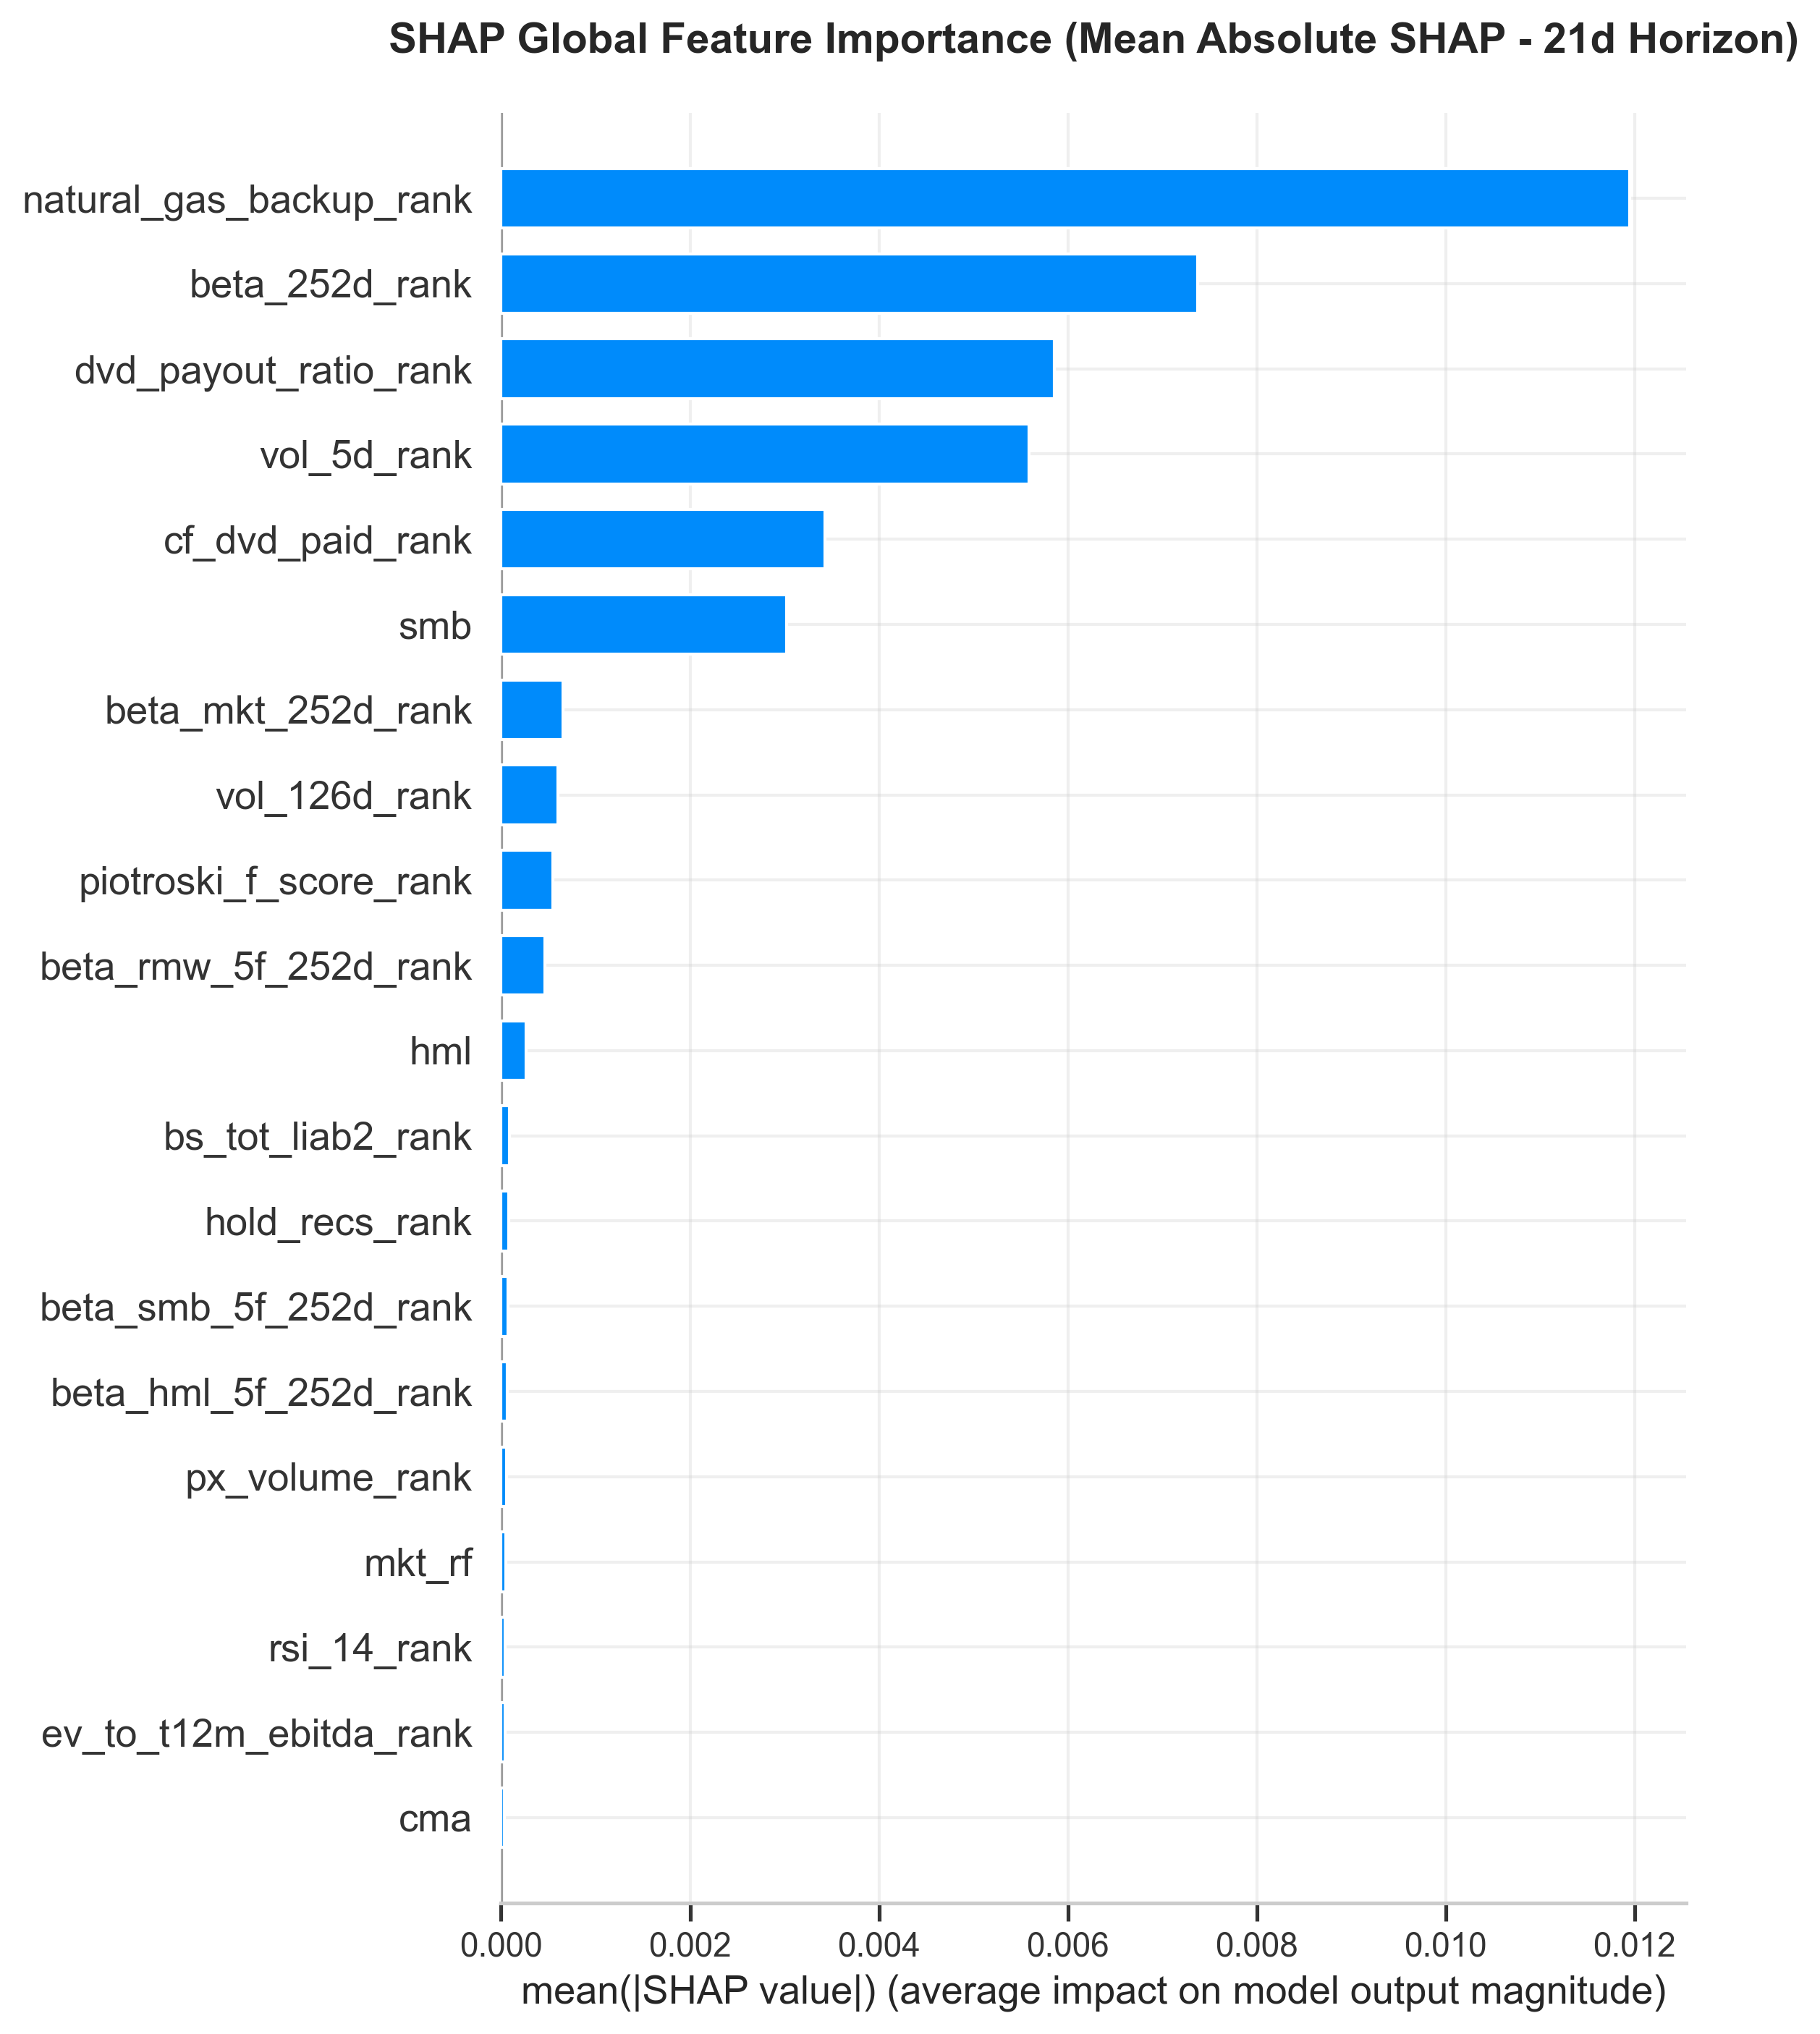
\includegraphics[width=0.85\textwidth]{figures/shap_bar_plot_21d_feattech_fund.png}
\caption{Global SHAP Mean Absolute Feature Importance Rankings (21-Day Horizon)}
\label{fig:ch5_shap_bar}
\end{figure}

\begin{figure}[H]
\centering
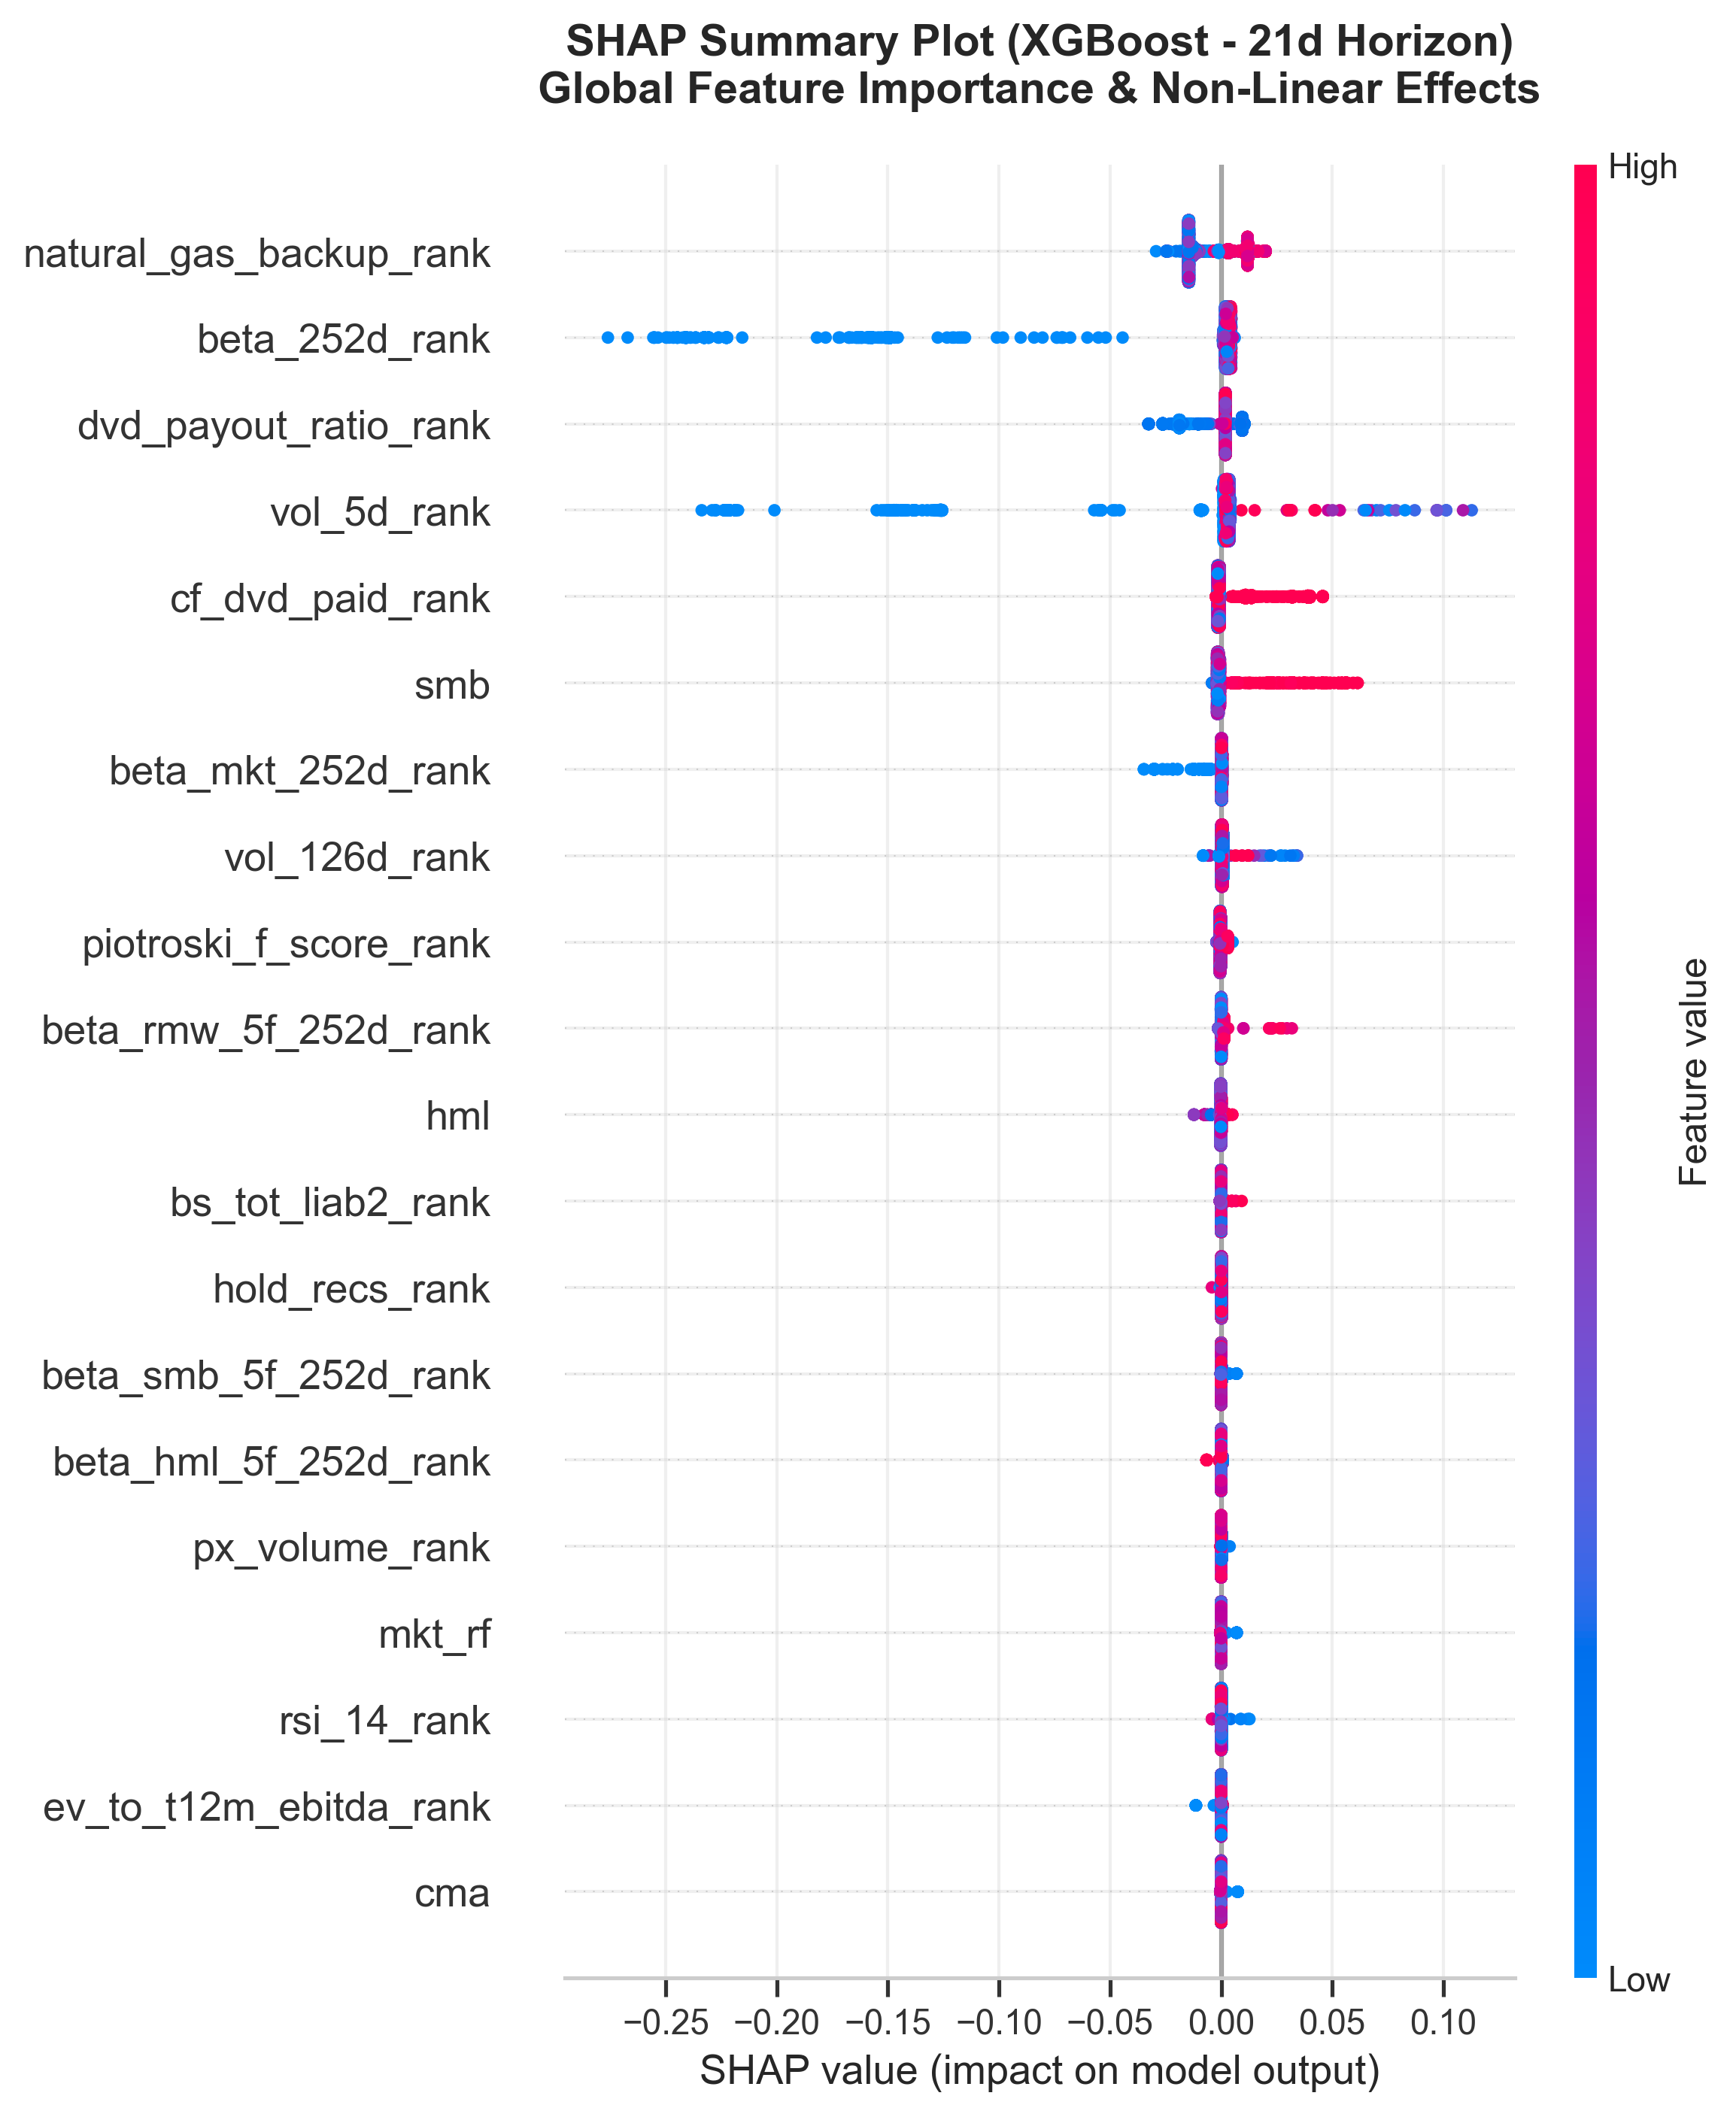
\includegraphics[width=0.85\textwidth]{figures/shap_summary_plot_21d_feattech_fund.png}
\caption{SHAP Summary Beeswarm Plot Illustrating Feature Value Impact on Model Predictions}
\label{fig:ch5_shap_summary}
\end{figure}

My SHAP analysis indicates that short term price momentum (\texttt{mom\_21d\_rank}) and relative strength (\texttt{rsi\_14d\_rank}) drive high-frequency predictive directionality \citep{jegadeesh1993returns, carhart1997on}, while quarterly fundamental operating quality (\texttt{quality\_proxy\_rank}) and valuation metrics (\texttt{value\_proxy\_rank}) provide structural drawdown defense during market contractions \citep{novy2013other, fama2015five}.
